\section{Collision Avoidance} \label{sec:collision_avoidance}
% \subsection{Inertia Drift}
% Let us assume that have strong damping in the direction of the obstacle, i.e., $s^{\mathrm{obs}} / m_i \gg 1$, where $m_i$ with $i = 1, .., N$ represent the eigenvalues of the mass matrix $\matd{M}$. 

\subsection{Disturbance Repulsion}
While the system is passive, it is important to analyze the behavior with respect to obstacles. For this we want to show what velocities can be absorbed based on the proposed controller design.

Let us assume a disturbance impact at time $t_0$, which results in the robot having a velocity of $\vecs{\dot \xi} = \vect f(\vecs \xi) + \vect v^I$, which is pointing towards the obstacle (see Fig.~\ref{fig:disturbance_with_parallel_velocity}). As we assume a large impact velocity, we consider that the obstacle is locally flat and the initial velocity constant and parallel to the surface. Furthermore, we assume to be close to the robot, i.e., $\Gamma(\vecs \xi) \approx 1$, hence the $w(\vecs \xi) \approx 1$, and the damping in the direction of the obstacle is approximated as $s^{\mathrm{obs}}$.
We further assume that the Coriolis effect can be neglected due to the small motion of the agent.

\begin{lemma}
	Let us consider a dynamical system that evolves according to the rigid body dynamics given in \eqref{eq:robot_dynamics} and is governed by the obstacle aware, passive controller \eqref{eq:control_command}, using the damping matrix $\matd{D}$ as defined in \eqref{eq:damping_summation}.
	A motion starting in free space, i.e., $\Gamma( \{\vecs \xi_0 \} ) > 1$ is able to reject disturbance and remain collision free for all times $\Gamma( \{\vecs \xi_t\}) \geq 1$ with $t \geq 0$ if the impact velocity is limited as follows $\| \vect v^I \| < s^{\mathrm{obs}} \| \vecs \xi - \vecs \xi^b \| / m$.
\end{lemma}

\begin{figure}[htb]
\centering
 % \begin{subfigure}{0.99\columnwidth}
  \centerline{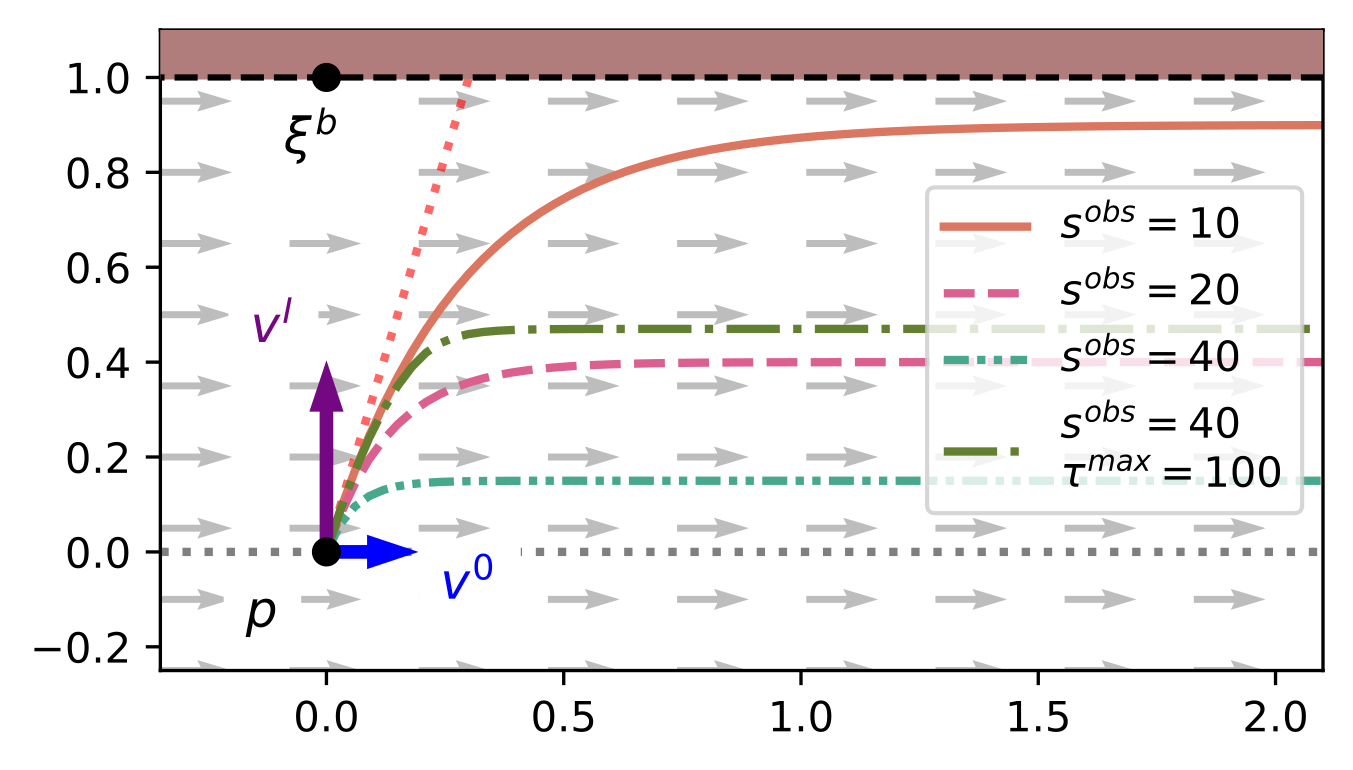
\includegraphics[width=0.99\columnwidth]{figures/parallel_avoidance_obstacle}}
  \caption{Disturbance rejection of an impact in the direction of the velocity.}
  \label{fig:disturbance_with_parallel_velocity}
% \end{subfigure}
\end{figure}

\begin{proof}
When approaching the obstacle $\| \vecs \xi - \vecs \xi^b \| \ll 1$ with a finite surface curvature, are assumed to be locally constant $\vect f(\vecs \xi)$. Furthermore, they are parallel or point away from the surface normal, i.e., $\dotprod{\vect f(\vecs \xi)}{\vect n(\vecs \xi)} \geq 0$.

Using \eqref{eq:control_command}, the velocity evolves as follows:
\begin{equation}
    \vecs{\dot \xi} = \int \vecs{\ddot \xi} \, dt = \int \matd{M}^{-1} \matd{D}  
	\left( \vecs{\dot \xi} - \vecs f(\vecs \xi) \right) \, dt
\end{equation}

Due to the proximity to the obstacle, we have from \eqref{eq:damping_summation} the weight being $w(\vecs \xi) = 1$. Hence, for the most critical scenario, where the disturbance is towards the obstacle, the velocity evolves as:
\begin{equation}
    \vecs{\dot \xi} = \int \frac{s^{\mathrm{obs}}}{m} \vecs{\dot \xi} \, dt = \frac{s^{\mathrm{obs}}}{m} (\vecs{\xi} - \vecs \xi_0)  + \vecs v^I \label{eq:velocity_with_control}
\end{equation}
where $m = \min \Bigl(\text{eig} \bigl(\mathcal{M} \bigr) \Bigr)$ is the smallest eigenvalue of the mass matrix 
Note, that any velocity which does not point towards the surface, will not get as close to the obstacle.

This can be used to compute the distance at which the velocity reaches zero:
\begin{equation}
    \| \vecs{\dot \xi} \| = 0
    \quad \Rightarrow \quad
    \|\vecs \xi_0 - \vecs{\xi} \| = \| \vecs v^I \| {m} / {s^{\mathrm{obs}}} 
\end{equation}

Hence, if starting at a position that is further away or at an equal distance, a disturbance velocity of $\vect v^I$ can be rejected, see Figure~\ref{fig:disturbance_with_parallel_velocity}.
\end{proof}

Note as the analysis is done for proximity regions of the obstacle. For a collision to occur, the robot would have to enter this proximity region. Hence, the proposed controller is able to reject a general impact for any region.

The above analysis has been specifically for disturbance velocities, yet, a system is disturbed by a force. The corresponding disturbance velocity is obtained by integrating the force over time (considering the mass matrix, too). 
Note, that the proposed controller is not able to actively reject a continuous force. 
However, this could be achieved by designing the dynamics $\vect f(\vecs \xi)$ to point away from the surface, as is proposed in \cite{huber2023avoidance}.

\subsection{Disturbance Repulsion with Force Limit}
All robotic systems have a maximum force that they  exerted based on the motors and their geometry, $\tau_c^{\mathrm{max}} \in \mathbb{R}_{>0}$. Note, such a force might be state dependent.

A limiting force increases the impact velocity $\vect v^I$ a controller is able to handle to ensure collision avoidance, see Fig.~\ref{fig:disturbance_with_parallel_velocity}. Nevertheless, a maximum control force can be interpreted as an adapting damping parameter, and hence the passivity from Theorem~\ref{theorem:passivity} still holds.

% Such a force, can result in an increase of tmaximum impact velocity 
% Let  us assume strong damping concerning the maximum force, i.e., $s^{\mathrm{obs}} / \tau_c^{\mathrm{max}} \gg 1$, hence we can assume that the magnitude of the obstacle repulsive force is equal to the maximum force close to the obstacle. Hence, the maximum disturbance.

% \subsection{Practical Considerations}
% As described in \cite{huber2022avoiding, huber2023avoidance}, the avoidance velocity when approaching an obstacle can be directed along the normal of the obstacle to point away from the surface when reaching the obstacle and inside. This allows improved recovery, for scenarios such as those presented.


